\section{Smart energy management}
This characteristic has two main functionalities:
\begin{enumerate}
\item If a window is opened when the heaters are working,this window will be closed automatically.
\item The daily schedule of each inhabitant is stored in a XML file. In the periods of the day when the house is empty, the heaters are disconnected and reconnected with enough time to reach the desired temperature when the inhabitants come back home.
\end{enumerate}
To activate this characteristic, go to the smartEnergy tab and click on the red button.
\begin{center}
	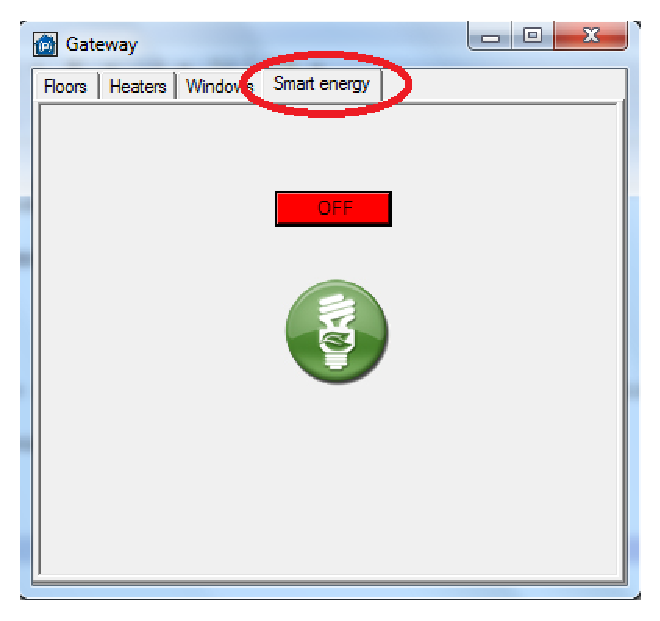
\includegraphics[width=.75\linewidth]{images/globalSmartEnergy.eps}
	\\
\vspace{1cm}
\end{center}
When this characteristic is on, you can establish the desired temperature. This temperature is used to reach an adequate temperature when the house is empty. To modify the temperature value, write your desired value and click on the button called \emph{Submit}.
\begin{center}
	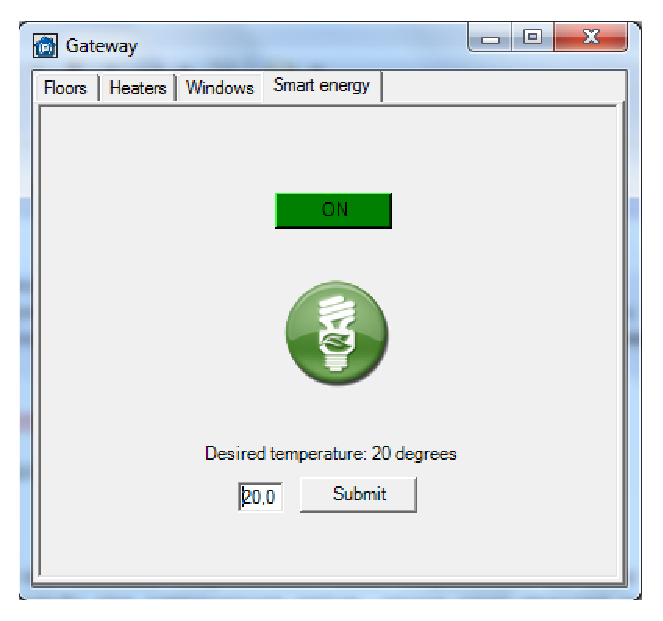
\includegraphics[width=.75\linewidth]{images/desiredTemperatureSmartEnergy.eps}
	\\
\vspace{1cm}
\end{center}
In the file \emph{timetable.xml} of your project, you can find the daily schedule of all inhabitants. If you want to change it, open it and modified tags. The tag called \emph{timetable} contains the hours where this inhabitant is outside of the house.
\begin{center}
	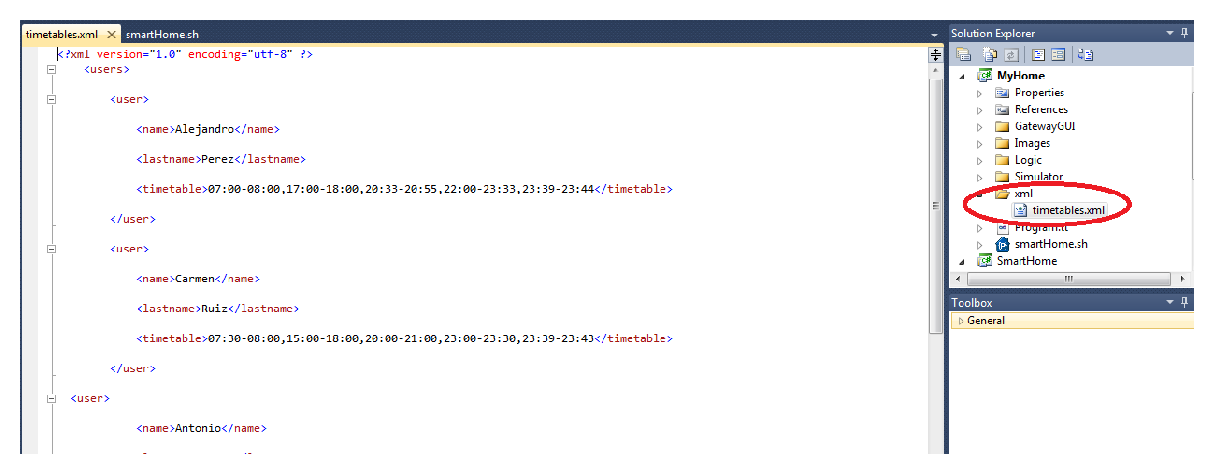
\includegraphics[width=.99\linewidth]{images/xmlSmartEnergy.eps}
	\\
\vspace{1cm}
\end{center}

In the tag called SmartEnergy in the Simulator window, you can find a list where you can see the hours when the house is empty. And you can change the current system time, so if you establish a time which nobody is in the house, all the heaters will be disconnected, unless the time is close to come back a inhabitant.
\begin{center}
	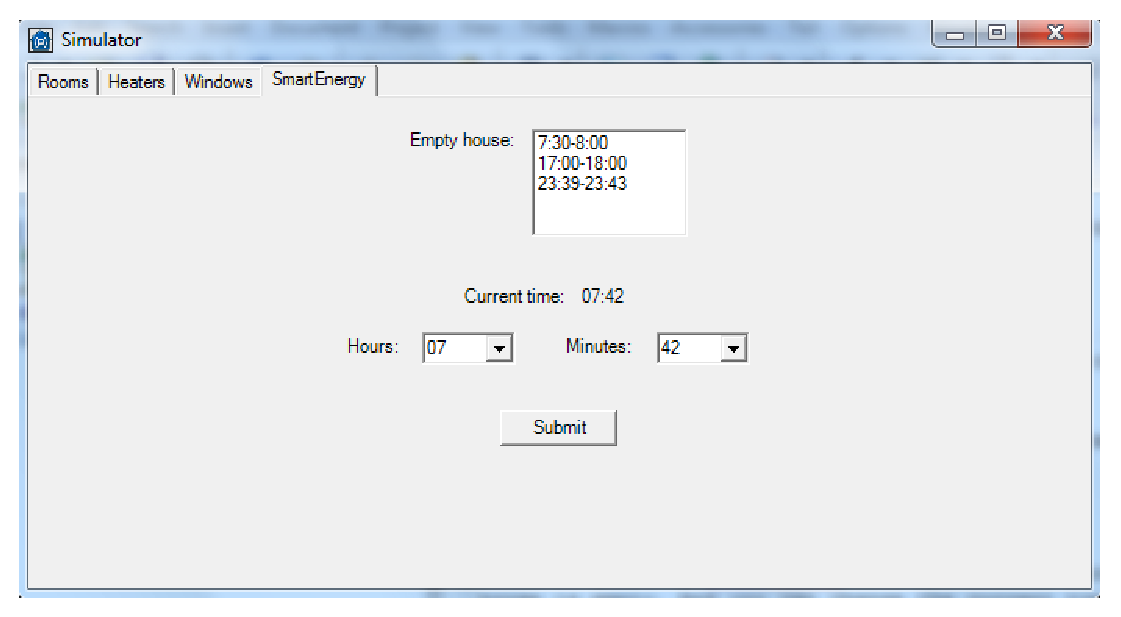
\includegraphics[width=.99\linewidth]{images/simulatorSmartEnergy.eps}
	\\
\vspace{1cm}
\end{center}
